\documentclass[tikz, border=10pt]{standalone}
\usetikzlibrary{positioning, arrows.meta, calc}
\usepackage{luatexja-fontspec}
\setmainjfont{HiraMaruProN-W4} % ヒラギノ丸ゴシックを指定

\begin{document}
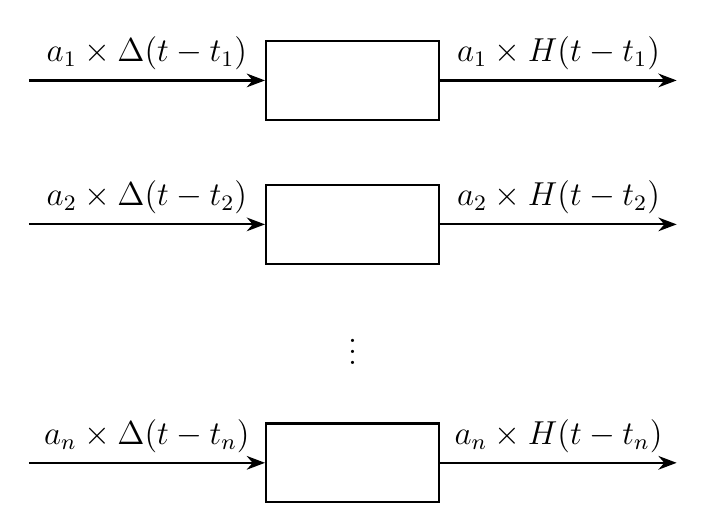
\begin{tikzpicture}[
    thick,                  % 線を太めにする
    >=Stealth,              % 綺麗な矢じりを使用
    font=\large,            % フォントサイズを一括で大きくする
    block/.style={draw, rectangle, minimum width=2.2cm, minimum height=1cm},
    node distance=0.8cm     % 1番と2番の間隔を適切な 0.8cm に固定
]

    % --- 1段目 (t_1) ---
    \node [block] (sys1) {};
    \draw [->] (sys1.west) ++(-3.0,0) -- (sys1.west) node[midway, above] {$a_{1}\times\Delta(t-t_1)$};
    \draw [->] (sys1.east) -- ++(3.0,0) node[midway, above] {$a_{1}\times H(t-t_1)$};

    % --- 2段目 (t_2) ---
    % 1つ目のboxから 0.8cm 下に配置（あきすぎを解消）
    \node [block, below=of sys1] (sys2) {};
    \draw [->] (sys2.west) ++(-3.0,0) -- (sys2.west) node[midway, above] {$a_{2}\times\Delta(t-t_2)$};
    \draw [->] (sys2.east) -- ++(3.0,0) node[midway, above] {$a_{2}\times H(t-t_2)$};

    % --- n段目 (t_n) ---
    % リーダーの上下にそれぞれ「0.8cmずつの隙間」を作るため、
    % 2つ目のboxの底から【0.8cm（上隙間） + リーダーの高さ（約0.4cm） + 0.8cm（下隙間）】を計算し、
    % ちょうど良い距離（2.0cm）下に3つ目のboxを配置します。
    \node [block, below=2.0cm of sys2] (sysn) {};
    \draw [->] (sysn.west) ++(-3.0,0) -- (sysn.west) node[midway, above] {$a_{n}\times\Delta(t-t_n)$};
    \draw [->] (sysn.east) -- ++(3.0,0) node[midway, above] {$a_{n}\times H(t-t_n)$};

    % --- 3つの点（縦の三点リーダー） ---
    % 2段目とn段目の隙間の「ちょうど真ん中」に配置することで、上下に均等な隙間が生まれます
    \node at ($(sys2.south)!0.5!(sysn.north)$) {$\vdots$};

\end{tikzpicture}
\end{document}

